\section{Our Approach}
\begin{frame}{Our Approach}
    \begin{description}
    \item[\acs{approachname}] \acl{approachname}
    \end{description}
    
    \only<1>{
        \begin{figure}[htbp]
        \centering
            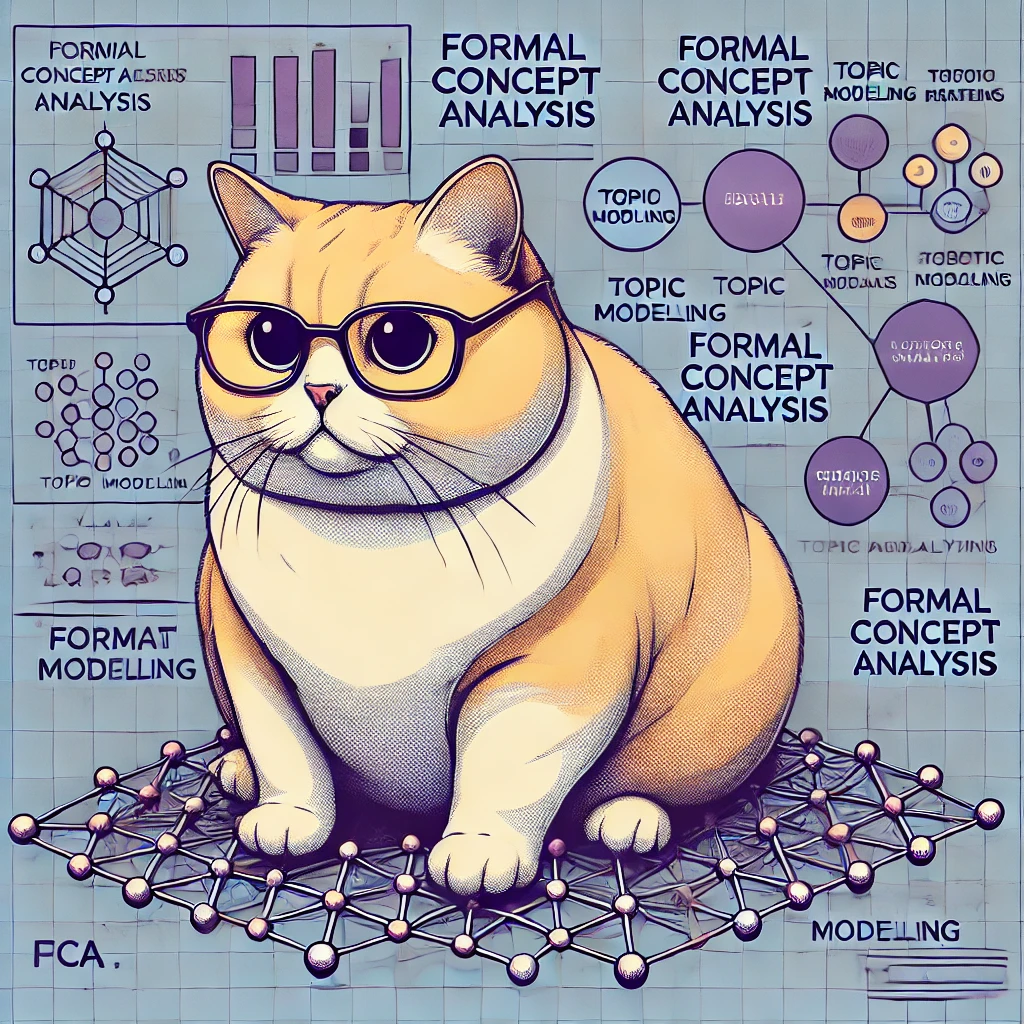
\includegraphics[height=0.6\textheight]{images/DALLE_2025_02_21_fat_cat.png}
        \label{fig:fat_cat}
    \end{figure}
    \begin{center}
        \scriptsize Image generated by DALLE (February 21, 2025)
    \end{center}
    }

    \only<2->{
        \begin{figure}[htbp]
        \centering
        \scalebox{0.9}{
            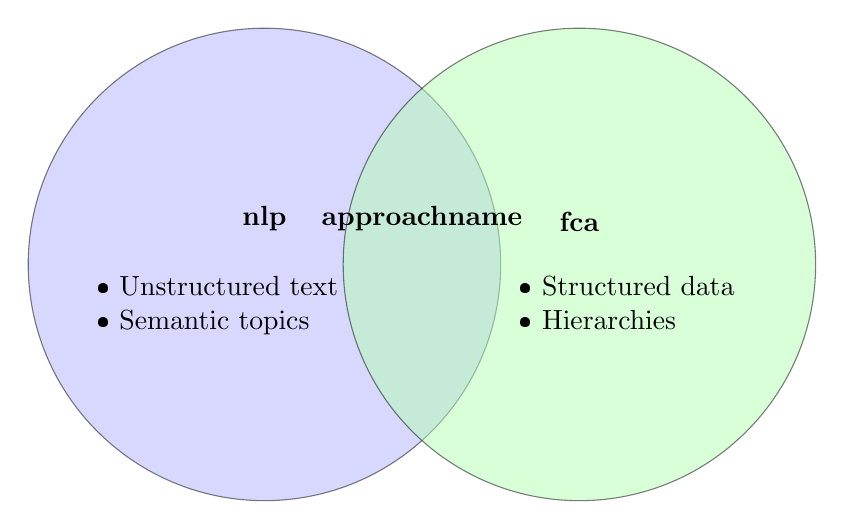
\begin{tikzpicture}
                 % Draw circles
                \draw[fill=blue!30, opacity=0.5] (-2,0) circle (3);
                \draw[fill=green!30, opacity=0.5] (2,0) circle (3);

                % Labels above circles
                \node[above] at (-2,0.3) {\textbf{\acs{nlp}}};
                \node[above] at (2,0.3) {\textbf{\acs{fca}}};
                \node[above] at (0,0.3) {\textbf{\acs{approachname}}};

                % NLP-only contributions (inside left circle, lower)
                \node[align=left] at (-2.6,-0.7) {
                    \textbullet\ Unstructured text\\
                    \textbullet\ Semantic topics\\
                    % \textbullet\ Statistical\\
                };

                % FCA-only contributions (inside right circle, lower)
                \node[align=left] at (2.6,-0.7) {
                    \textbullet\ Structured data\\
                    \textbullet\ Hierarchies\\
                    % \textbullet\ Deductive reasoning\\
                };
            \end{tikzpicture}
        }
        \label{fig:venn_nlp_fca}
    \end{figure}
    }

\end{frame}

\begin{frame}{Our Approach}
    \begin{description}
    \item[\acs{approachname}] \acl{approachname}
    \end{description}

    Our contributions:
    \begin{itemize}
        \uncover<2->{\item Open-source\footnote{\url{https://github.com/KlaraGtknst/text_topic} (29.01.2025) \&\\ \url{https://github.com/KlaraGtknst/clj_exploration_leaks} (29.01.2025)}}
        \uncover<3->{\item Minimal training requirements}
        \uncover<4->{\item Non-textual data} % \item[\rightarrowfill]
        \uncover<5->{\item Information aggregation across directories}       
    \end{itemize}
\end{frame}

\begin{frame}{Text Extraction}
    \includesvg[width=\linewidth]{images/extract_text}
    \label{fig:extract_text}
    \begin{beamercolorbox}[center, wd=\linewidth, sep=1ex, rounded=true, shadow=true]{block body}
        {\small Appendix details: } 
        \hyperlink{supp:img_cap}{\beamergotobutton{Image Captioner}}
    \end{beamercolorbox}
\end{frame}


% \begin{frame}{Text Processing}
%     \includesvg[width=\linewidth]{images/text_related_workflow}
%       \vfill
%     \begin{beamercolorbox}[center, wd=\linewidth, sep=1ex, rounded=true, shadow=true]{block body}
%         {\small Appendix details: } 
%         \hyperlink{supp:img_cap}{\beamergotobutton{Image Captioner}}
%         \hspace{1em}
%         \hyperlink{supp:sbert}{\beamergotobutton{\acs{sbert}}}
%     \end{beamercolorbox}
% \end{frame}

\begin{frame}{Deriving the Directory-Topic Concept Lattice}
    \only<1>{
    \includegraphics[width=\linewidth]{images/topic_modeling_fca_2rows.pdf}
    }
    \visible<2->{Assuming all documents are organized in directories.}
    \begin{enumerate}
        \item <2-> Top 10 topics per document incl. relevance scores
        \item <3-> Compute threshold $\delta$ s.t. document-topic matrix density $< 0.1$
        \item <4-> $\mathcal{D}_\delta(i,j)=\left\{ \begin{array}{cl}
                        1 & \ \text{if } \ w_{i,j} \geq \delta, \\
                        0 & \ \text{else.}
                    \end{array} \right.$
        \item <5-> Compute iceberg lattice for each directory
        \item <6-> Combine frequent topics across directories into directory-topic matrix
        \item[\rightarrowfill] <7-> Directory-topic context
    \end{enumerate}


    \only<3>{
        \centering
        \includesvg[width=0.6\linewidth]{images/Density_of_document_topic_incidence_matrix_altered}
    }

  \only<4>{
    \begin{center}
        \captionof{table}{Document-topic relation $\mathcal{D}_\delta$~\cite{topic_modeling_2024}}
        \label{tab:doc-topic2}
        % \resizebox{\linewidth}{!}{%
            \begin{tabular}{|c|c|c|c|c|}
                \hline
                \diagbox{Documents}{Topics} & $t_1$ & $t_2$ & $\cdots$ & $t_n$ \\ \hline
                $d_1$ & $w_{1,1}$ & $w_{1,2}$ & $\cdots$ & $w_{1,n}$ \\ \hline
                $d_2$ & $w_{2,1}$ & $w_{2,2}$ & $\cdots$ & $w_{2,n}$ \\ \hline
                $\vdots$ & $\vdots$ & $\vdots$ & $\ddots$ & $\vdots$ \\ \hline
                $d_l$ & $w_{l,1}$ & $w_{l,2}$ & $\cdots$ & $w_{l,n}$ \\ \hline
            \end{tabular}
        % }
        \end{center}
    }


    \only<5>{
        \begin{center}
            \resizebox{0.25\linewidth}{0.3\textheight}{%
                \FormalConceptGraphColoured
            }

            \vspace{0.5em}
            {\scriptsize Iceberg concept lattice coloured.}
        \end{center}
    }


    \visible<6>{
        \begin{table}[t]
    \centering
    \caption{Weighted directory-topic relation.
        The weights $\tilde{w}_{i,j} \in \{0,1\}$ represent whether a topic $t_j$ is present in a directory $\hat{d}_i$.}
    \label{tab:dir-topic}
    \begin{tabular}{|c|c|c|c|c|}
        \hline
        \backslashbox{Directories}{Topics} & $t_1$             & $t_2$             &          & $t_n$             \\ \hline
        $\hat{d}_1$                        & $\tilde{w}_{1,1}$ & $\tilde{w}_{1,2}$ & $\cdots$ & $\tilde{w}_{1,n}$ \\ \hline
        $\hat{d}_2$                        & $\tilde{w}_{2,1}$ & $\tilde{w}_{2,2}$ & $\cdots$ & $\tilde{w}_{2,n}$ \\ \hline
        $\vdots$                           & $\vdots$          & $\vdots$          & $\ddots$ & $\vdots$          \\ \hline
        $\hat{d}_k$                        & $\tilde{w}_{k,1}$ & $\tilde{w}_{k,2}$ & $\cdots$ & $\tilde{w}_{k,n}$ \\ \hline
    \end{tabular}
\end{table}
    }
\end{frame}
